\documentclass{jarticle}
\usepackage{rsj}
\usepackage[dvips]{graphicx}
\usepackage{url}
\usepackage{bm}
\usepackage{amsmath}
\usepackage{amssymb}

\begin{document}
\title{Motion Primitive with Aerial Manipulator for Dynamic Tennis Swing Motion}
\author{Fan Shi\ \ Moju Zhao\ \ Tomoki Anzai\ \ Xiangyu Chen\ \ Kei Okada\ \ Masayuki Inaba}

\setlength{\baselineskip}{4.4mm}
\maketitle
\thispagestyle{empty}
\pagestyle{empty}

\section{Introduction}

In this paper, we implement a rapid real-time motion planning algorithm with a novel type of aerial manipulator, and dynamic tennis swing motion is achieved as an example to show the feasibility of the algorithm. When planning the feasible trajectory, dynamic constraints of the robot, and position, velocity and acceleration in start and end points are considered. Thousands of motion primitives are generated online and the least-cost trajectory to follow is selected by trajectory selector.


\refeq{temp}
\reffig{abst-image}
Recently, aerial robots raise increasing attentions and lots of fundamental researches appear in geometric control, 3D mapping,  and real-time planning. With the help of these fundamental researches, aerial robots shows great potential to interact with environments and take more complex tasks such as multi-field drone, moving collaborate object. Among them, aerial manipulator is the most exciting and difficult one since it directly interact with the environments. Several researches of aerial manipulators are shown, some work attaches a high-DOFs robot arm to the downward base of the drone and more consideration in stability and workspace is needed\cite{aerial_manipulator_1}, some are a simple 1-DOF gripper with limited functions. Hence, our lab come up with a transformable drone (Hydrus) as the aerial manipulator with dual arms, which have lots of potentials like moving in clustered environments and moving heavy objects[3].

\begin{figure}[htb]
  \centering
  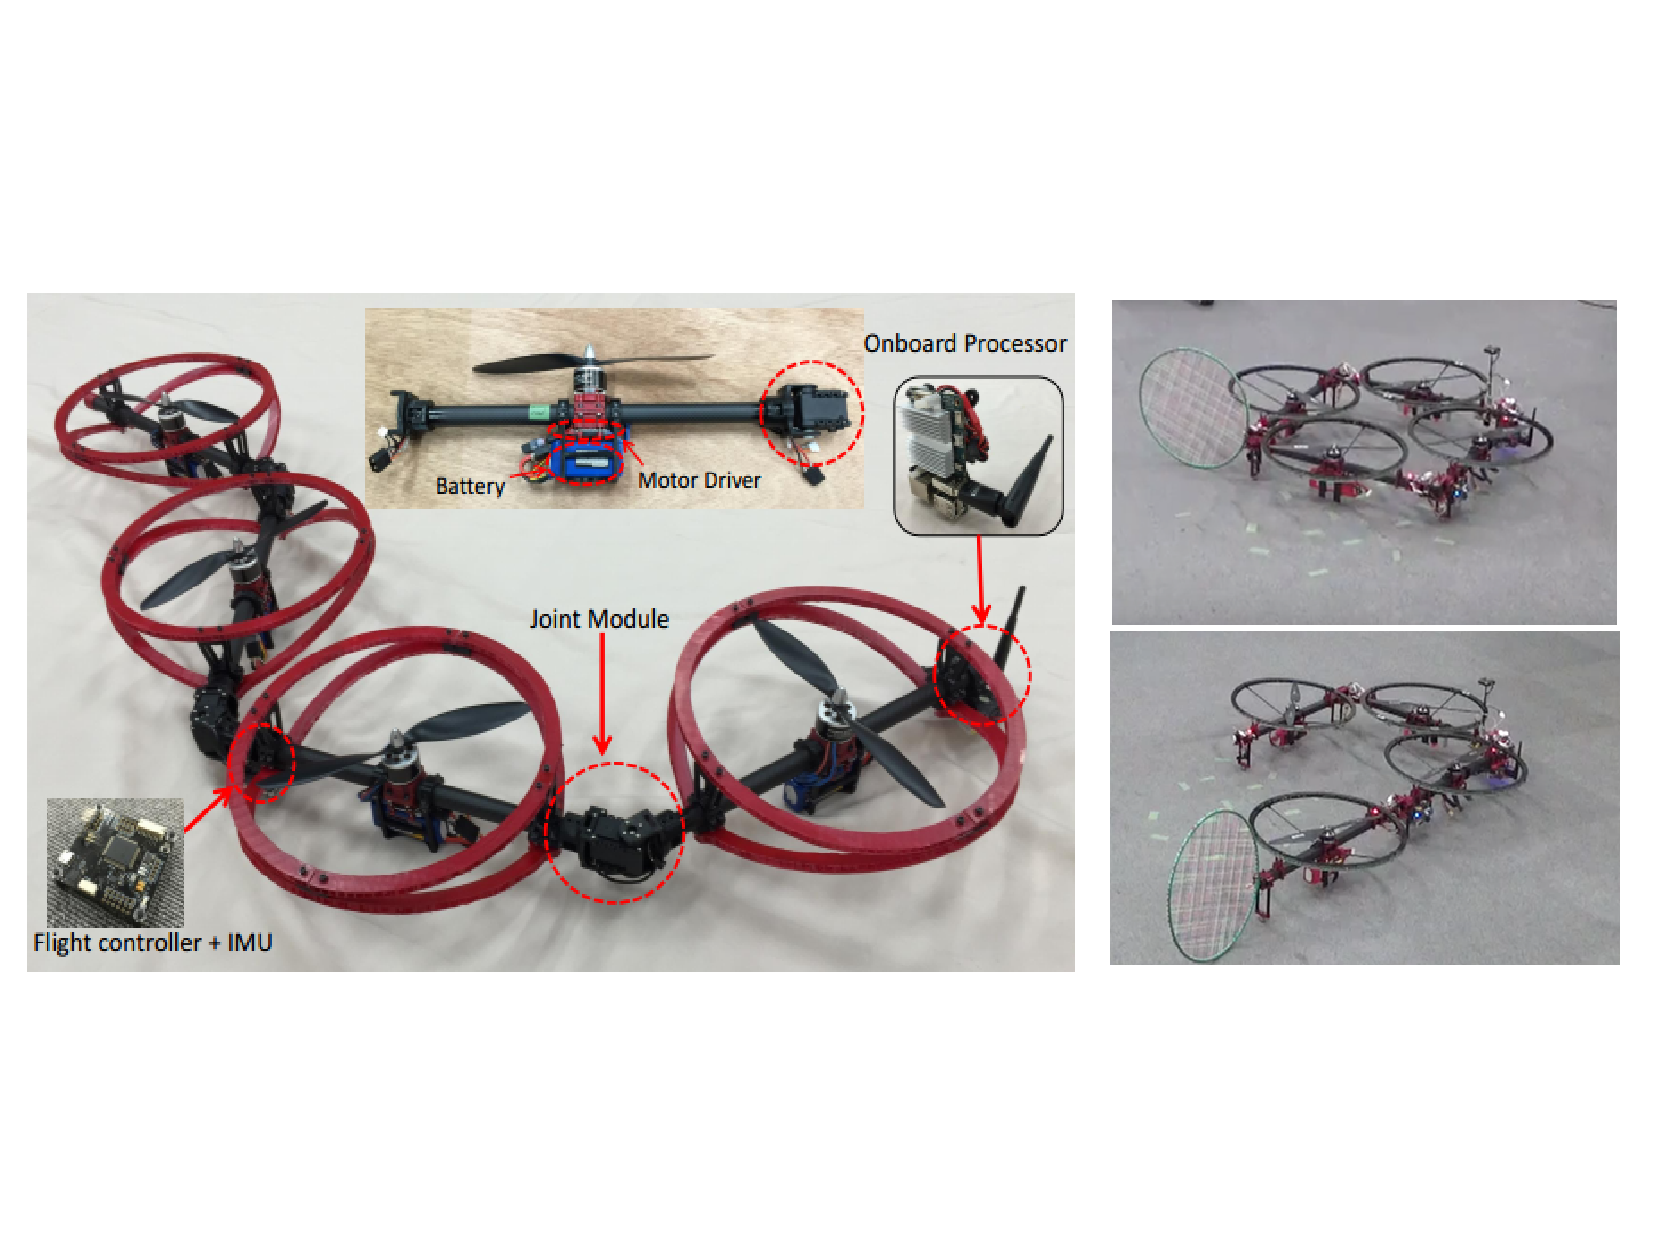
\includegraphics[clip, bb= 10 128 777 457,  width=\columnwidth]{figs_orig/figure.pdf}
  \caption{TODOTODO}
  \label{fig:abst-image}
\end{figure}

\section{Motion}


TODOTODOTODOTODOTODOTODO TODOTODOTODOTODOTODOTODO\cite{Morgan:ROS}
end.

\begin{equation}
  \label{eq:temp}
\bm{f}(t) = \left( \begin{array}{c}
  \bm{x}(t) \\
  \bm{v}(t) \\
  \bm{a}(t)
\end{array}\right)
\end{equation}

\begin{equation}
  \label{eq:temp2}
\bm{f}(t) = \left( \begin{array}{c}
  \bm{a}t^5 + \bm{b}t^4 + \bm{c}t^3 + \bm{d}t^2 + \bm{e}t + \bm{f} \\
  5\bm{a}t^4 + 4\bm{b}t^3 + 3\bm{c}t^2 + 2\bm{d}t + \bm{e} \\
  20\bm{a}t^4 + 12\bm{b}t^2 + 6\bm{c}t + 2\bm{d}
\end{array}\right)
\end{equation}


\begin{eqnarray}
  \label{eq:temp3}
 & min{\int_0^T |f^{(3)}_x(t) + f^{(3)}_y(t) + f^{(3)}_z(t)|^2 dt}   \\
  \label{eq:temp4}
s.t. &  V_{i_{min}} < f^{(1)}_i(t) < V_{i_{max}}, i = x, y, z \nonumber \\
  \label{eq:temp5}
 & a_{i_{min}} < f^{(2)}_i(t) < a_{i_{max}}, i = x, y, z \nonumber \\
  \label{eq:temp6} 
 & 0 < f_z(t) \nonumber
\end{eqnarray}


\begin{equation}
  \label{eq:temp7}
  C_{obstacle}\bigcap (f_x(t), f_y(t), f_z(t)) =\emptyset
\end{equation}


\section{TODOTODO}

\section{Simulation Result}


\section{Conclusion}


{\footnotesize
%\small
\bibliographystyle{junsrt}
\bibliography{main}
}
\end{document}
